\documentclass[11pt]{report}

%packages we want
\usepackage{hyperref}
\hypersetup{
    colorlinks,
    citecolor=black,
    filecolor=black,
    linkcolor=blue,
    urlcolor=blue
}
\usepackage{graphicx}
\DeclareGraphicsExtensions{.pdf,.png,.jpg}



%Some helpful commands
\newcommand{\csgt}[0]{\textbf{CS\textgreater\ }}

%Gummi|065|=)
\title{\textbf{\csgt System User Manual}}
\author{Jeb Brooks}
\date{}
\begin{document}

\maketitle

\tableofcontents

\chapter{Introduction}
The \csgt system is an all in one submission system and grading platform designed primarily for use
with CS coursework. It is designed to support basic grading functionality and auto-grading capabilities.
Additionally it is designed to be extended to support new testing systems through a simple plug-in system
which can hot-load new plugins on a live instance.

This document will attempt to get you familiar with the \csgt system and guide you through using and maintaining 
its various features. \csgt provides the following major features:

\begin{itemize}
\item Logical assignment/problem grouping
\item Fully featured grade-book system. Supports adding groups and columns to the grade-book which are not
based on student submitted work (e.g.. Participation Points or Quizzes)
\item Markdown enabled grader comment system.
\item Automatic grading based on unit tests (modifiable via plug-ins)
\item Automatic late grade calculation (modifiable via plug-ins)
\item Built-in wiki support for problem descriptions and notes for graders. The wiki also supports various
permissions levels.
\item Support for command line control of the system.
\item Support for listing currently active tutors and locations so students can get help on problem sets.
\end{itemize}

This document will attempt to guide you through the use of these features. Because not all features are useful to
every class of user this document is divided into three chapters. The \nameref{ch:use} chapter should be 
enough for instructors, tutors, and students. The \nameref{ch:admin} chapter will cover topics required to set-up
and maintain the \csgt system. Finally, the \nameref{ch:develop} chapter will cover topics required to develop
new plug-ins and modify the core functionality of the system.


\chapter{Basic Use}
\label{ch:use}
Foo

\chapter{Administration}
\label{ch:admin}
\section{Server Structure}
The \csgt system is designed to be modular and expandable as the number of users of the system grows. 
To accommodate this each of the five major components are designed to be operated as a separate server. 
The five components are:

\begin{enumerate}
\item Python-Flask Front-end Server
\item Python-Celery Grading Worker
\item File-system for submission storage (pick your favorite one)
\item MongoDB for storing grades
\item RabbitMQ for passing grading requests to workers
\end{enumerate}

In the most basic configuration, which is most useful for testing, all of the required components will be 
on one machine. As the requirement for redundancy and scalability increases components may be moved to 
separate servers and replicated. Figure \ref{fig:layout} shows one possible configuration of the servers
which provides redundancy on both the front and back end. It is important to note that a load-balancer is
required to support multiple front-ends.

\textbf{Note:} Currently even though MongoDB and rabbitMQ support distributed options the system has never 
been tested using that configuration. This is a feature which may be researched in the future if it becomes
needed.

\begin{figure}
\centering
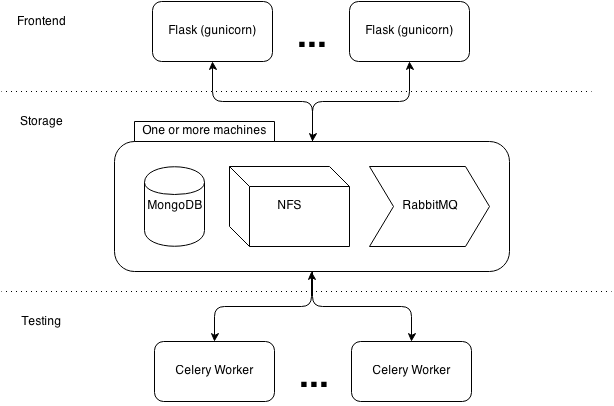
\includegraphics[width=\textwidth,height=\textheight,keepaspectratio]{diagrams/HMC_Grader_Layout}
\caption{Possible server configuration for \csgt}
\label{fig:layout}
\end{figure}


\section{Set-up}
Once you have decided on the basic configuration for your servers setting up the requisite systems requires a
little work. For each server type I will provide basic set-up instructions. These instructions are listed in 
order to prevent dependency issues. 

\subsection{MongoDB Set-up}
To set-up a brand new MongoDB instance you can use the instructions below. If you already have a running version
of MongoDB you can adapt the instructions or request help from your database administrator.
\begin{enumerate}
\item Get the latest version of MongoDB from \href{http://docs.mongodb.org/manual/tutorial/install-mongodb-on-ubuntu/}{here}.
\item Follow \href{http://docs.mongodb.org/manual/tutorial/enable-authentication/}{these} instructions to create an administrator account.
\item Edit \verb|/etc/mongodb.conf| so that 
\verb|bind_ip| is commented and uncomment
\verb|auth = true|. Additionally it is recommended to change the port that the server listens on
to prevent attacks.
\item Reload \emph{mongod} and log into the \emph{mongo} shell with\\
\verb|$ mongo -u {username} -p --authenticationDatabase admin|
\item Type \verb|use submissionsite| to create the \emph{submissionsite} database
\item Add a user for this database by typing
\begin{verbatim}
db.createUser(
  { user: "grader", 
    pwd: "{your password}",
    roles: [{role: "dbOwner", db: "submissionsite"}] 
  }
)
\end{verbatim}
\item Finally \verb|quit()| the mongo shell.
\end{enumerate}

\subsection{File-system Set-up}
Setting up the file-system is pretty easy. There are two major requirements for the file-system, one, it
must be accessible from all machines in the cluster, and two it must have a minimal required directory
structure.

Because exporting a directory is complicated and other better resources exist on the internet I leave
figuring out how to export your directory as an exercise to the reader.

Once you decide how to export your chosen storage directory you must give it some basic structure. This
structure is as follows:

\begin{itemize}
	\item submissions
	\item photos
	\item plugins
	\begin{itemize}
		\item autograder
		\item latework
	\end{itemize}
\end{itemize}

Once these paths exist in your storage directory you are good to go.

\subsection{RabbitMQ Set-up}

\chapter{Development}
\label{ch:develop}
Foo

\end{document}
